\chapter{Design}
Now, once planed "What" is the system, it is needed to plan the "How" the system will be build in 
the implementation fase. Here is explaned the components and the reason for it. As well
for the instructions on the system construction and realisation.

\section{Analysis Review}

Taking in account the limited personal and time, some of what is specified in Analysis
has the scope reduced as to accomplish acording to the requirements and constraints.
Using as inspiration the Copernicus SVP-BRST and the CMEMS labs previous experience,
the 5S can/ and will recall for used tecnology for easier design process.

The project then will be devided in three main parts; The Hardware, Software and the outer shell.
Then, lately, it will be shown the softwares used to accomplish this project. 

\section{Hardware}

This section elaborate on the system physical components, their connections and the 
reasons they ware chosen. It is important to remember that the main objective, even if 
it is not specified on the topic, is the lowpower functionalities. So the hability to
consume less power is a favoring point. 


\subsection{Autonomy}
Here will be discussed witch hardware is best sued for the task. The hardware will be evaluated by their
autonomy, the communication protocol

As for the autonomy there are two main factors to consider, the batteries and the board consumption
meaning that the whole system must consume, on average, 5mAH.
\subsubsection{Batteries}
Google sheets
\subsubsection{Board Consumption}

table

SIM7600 
table 6 and 34 (pg 20 and ) same voltage
2
SIM7020
peak 2A 20u in sleep mode 150mA

SIM7000 (GPS por NB-IoT e 2G fallback)
Consome: 11mA

SIM7080G - Nb-IoT
Quectel BG77

Quectel BG95-M3

 
GPS
MAX-M10S

tele2

IMU
BMI088 IMU Sensor
accelerometer 15uA  / and Gyroscope 2.7mA
ISM330BX
0.19mA / 0.6mA
activate BDU

BMI270


Unix Steptime

final list
IMU 9DOF GY-85 - ITG3205 + ADXL345 + HMC5883L
%final_IMU.png
\begin{figure}[H]
    \centering
    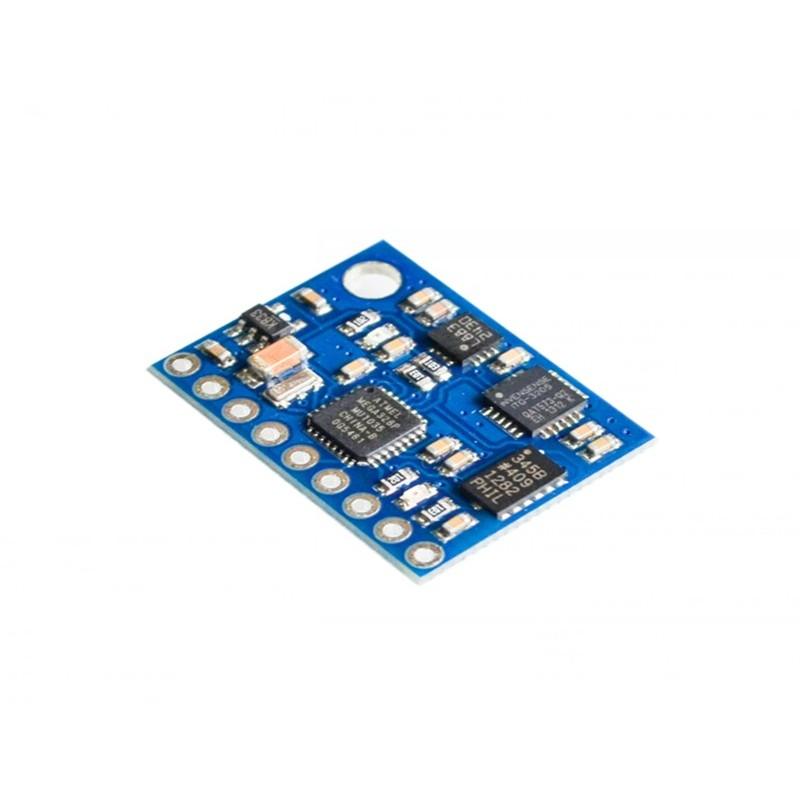
\includegraphics[width=0.75\textwidth]{images/chapter/design/components/final_IMU.png}  % Adjust the width as necessary
    \caption{Memory Flowchart}
    \label{fig:Memory Flowchart}        
\end{figure}

SIM7000E Arduino NB-IoT/LTE/GPRS/GPS Expansion Shield
%SIM7000.png

\begin{figure}[H]
    \centering
    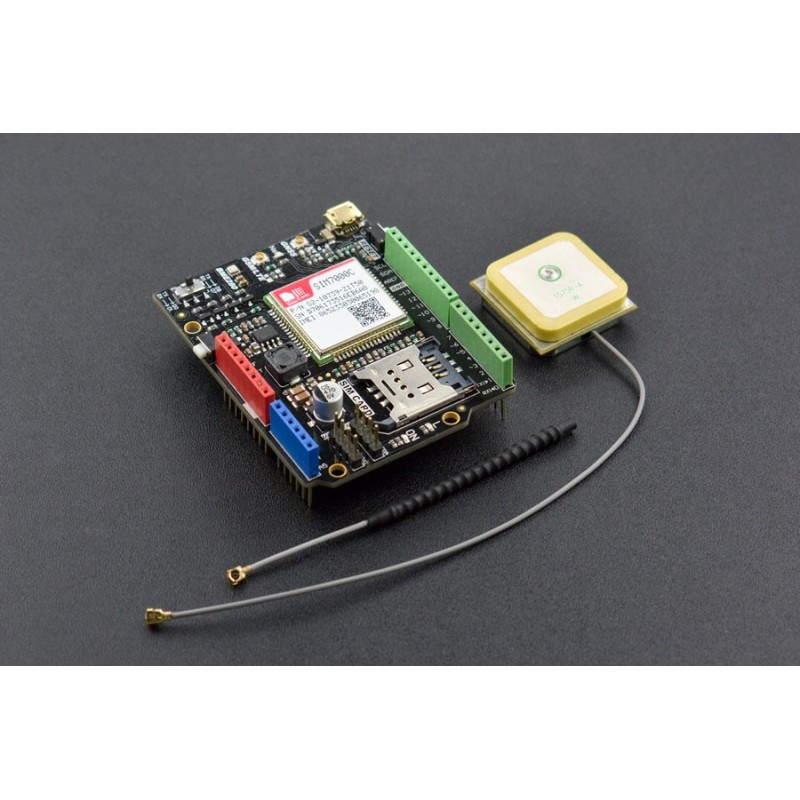
\includegraphics[width=0.75\textwidth]{images/chapter/design/components/SIM7000.png}  % Adjust the width as necessary
    \caption{Memory Flowchart}
    \label{fig:Memory Flowchart}        
\end{figure}

SENSOR DE TEMPERATURA À PROVA DE ÁGUA (DS18B20) 1M
%temp.png


\begin{figure}[H]
    \centering
    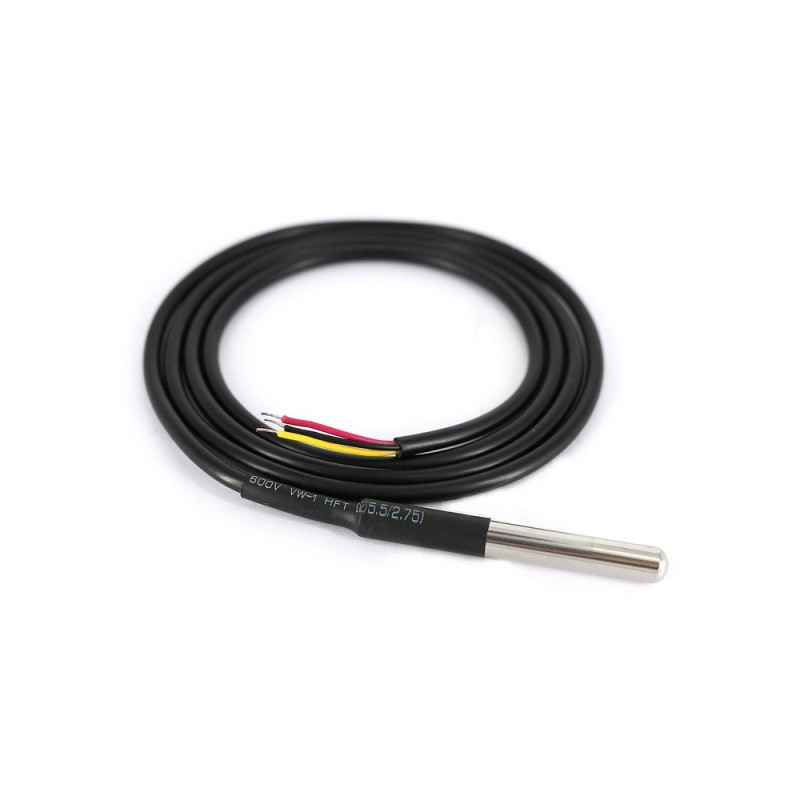
\includegraphics[width=0.75\textwidth]{images/chapter/design/components/temp.png}  % Adjust the width as necessary
    \caption{Memory Flowchart}
    \label{fig:Memory Flowchart}        
\end{figure}

Cartão micro SDHC 32GB Adata Class 10 UHS-I com adaptador
INF01016
%sdcard.png

\begin{figure}[H]
    \centering
    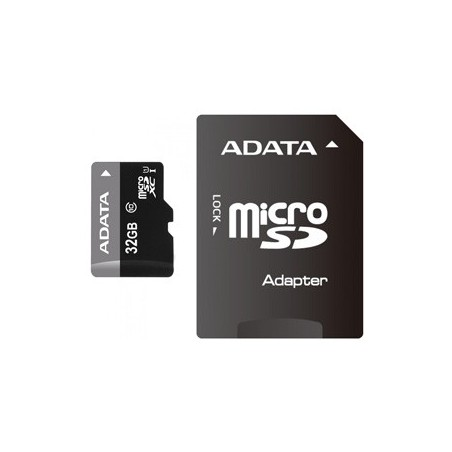
\includegraphics[width=0.75\textwidth]{images/chapter/design/components/sdcard.png}  % Adjust the width as necessary
    \caption{Memory Flowchart}
    \label{fig:Memory Flowchart}        
\end{figure}

Módulo leitor de cartões micro SD
%sd_support.jpg

\begin{figure}[H]
    \centering
    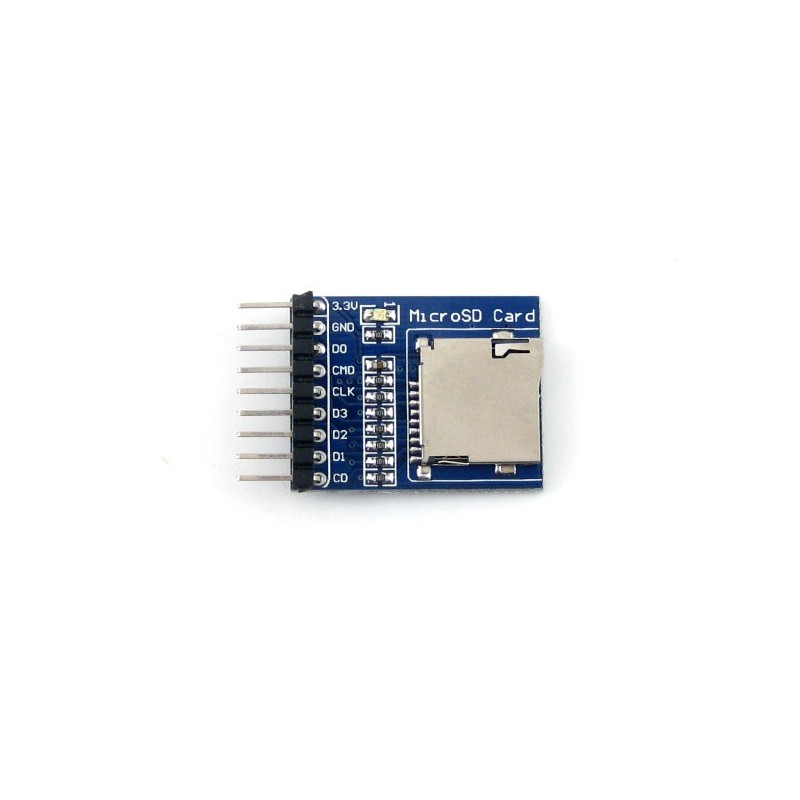
\includegraphics[width=0.75\textwidth]{images/chapter/design/components/sd_support.jpg}  % Adjust the width as necessary
    \caption{Memory Flowchart}
    \label{fig:Memory Flowchart}        
\end{figure}

Battery Holder for 4x 18650 with wires
%battery-holder.jpg

\begin{figure}[H]
    \centering
    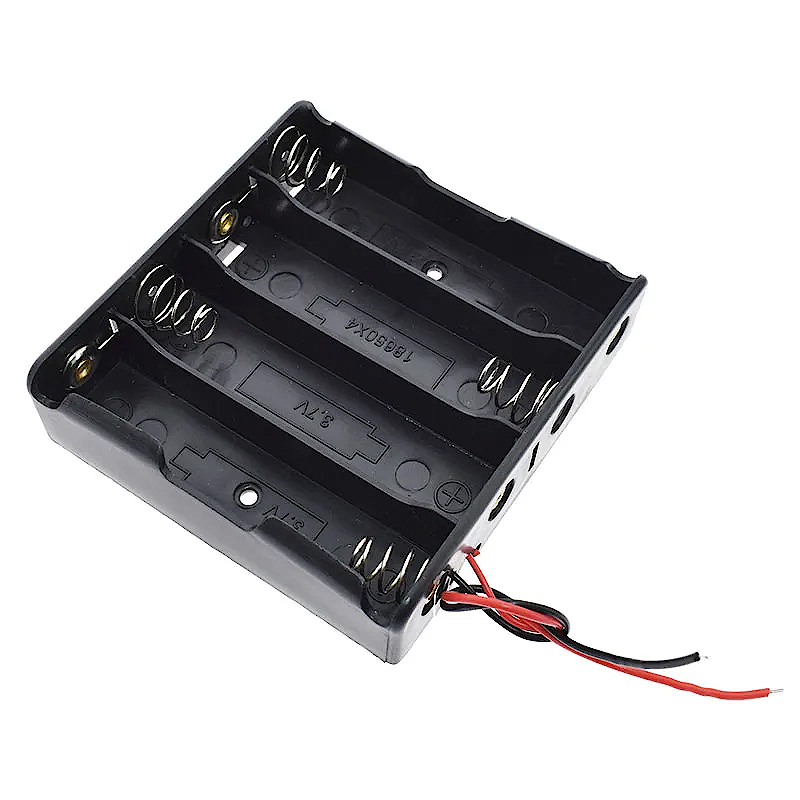
\includegraphics[width=0.75\textwidth]{images/chapter/design/components/battery-holder.jpg}  % Adjust the width as necessary
    \caption{Memory Flowchart}
    \label{fig:Memory Flowchart}        
\end{figure}

PILHA LI-ION 18650 3,7V 2000MAH
%batt.jpg

\begin{figure}[H]
    \centering
    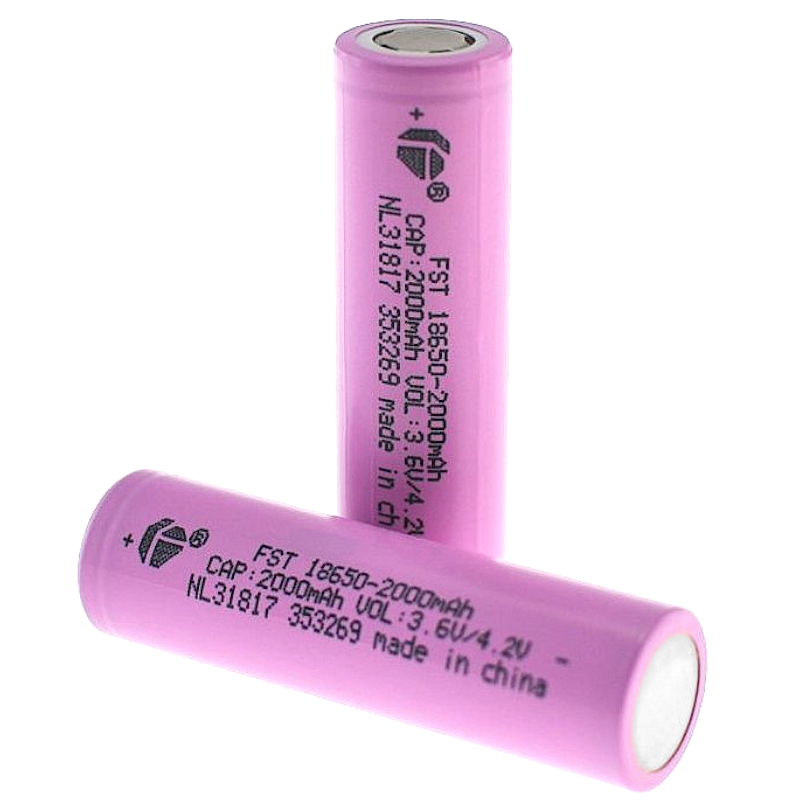
\includegraphics[width=0.75\textwidth]{images/chapter/design/components/batt.jpg}  % Adjust the width as necessary
    \caption{Memory Flowchart}
    \label{fig:Memory Flowchart}        
\end{figure}

Possible solar energy
solar penel
AEM10941
SM111K06L

\section{Hardware Specification}
\subsection{SDCard}
\subsection{STM32}

STM32L010K4T6
microcontroler
ADC
UART
SPI
ONEWire
\subsection{BMI088 IMU Sensor}
gyroscope and acelerometer


\subsection{Temperature}
DS18B20
\section{Software}

\subsection{Communication protocol}

factors to consider
chip
distance
bitrate
availability
table
EVKITST87M01-1 nb-iot
SIM7600 2g 3g 4g LTE CAT4

simbase chip availability

\begin{table}
    \centering
    \begin{tabular}{lllllll}
    Portugal & 2G & 3G & 4G & 5G & LTE & NB-IoT   \\
    Meo      & V  & V  & V  & -- & --  & --       \\
    Nos      & V  & V  & -- & -- & --  & --       \\
    Vodafone & V  & -- & V  & V  & V   & -- 
    \end{tabular}
\end{table}

europe coast
2g 4g


\section{Shell}
2.5 dB Antenna should be at least 10 cm form water 


\subsection{Conclusion}
\section{Case Construction}

Diagram


The hardware configurations, as idicated on the datasheet should follow the leading steps.
%hw config

As for the UART communication, the list of commads are listed on the datasheet. 
As for better flow, here are listed the commadsused along the project and their functionalities. 
%commmand list



\section{Tools and COTS}
\subsection{Tools}
\subsection{COTS}
\subsubsection{GPS and 4G module}
\subsubsection{Inkscape}
\subsubsection{draw.io}
\subsubsection{STM32 CUBEmx}
\subsubsection{\LaTeX}
\section{Software Specification}
\section{Theorical Concepts}